\documentclass[12pt]{article}
\usepackage{geometry}
\geometry{
	left=20mm,
	top=20mm,
}
\usepackage[utf8]{inputenc}
\usepackage[shortlabels]{enumitem}
\usepackage{array}
\newcolumntype{C}[1]{>{\centering\let\newline\\\arraybackslash\hspace{0pt}}m{#1}}
\usepackage[spanish,es-nodecimaldot]{babel}
 \usepackage{url}
 \usepackage{hyperref}
 \hypersetup{
 	colorlinks=true,
 	linkcolor=blue,
 	filecolor=magenta,      
 	urlcolor=cyan,
 }
 
 \urlstyle{same}
\usepackage[spanish, fixlanguage]{babelbib}
\bibliographystyle{IEEEtran}
\usepackage{graphicx}
\graphicspath{ {./images/} }
\usepackage{amssymb}
\usepackage{amsmath}
\usepackage{subcaption}
\usepackage[linesnumbered]{algorithm2e}
\newcommand\mycommfont[1]{\footnotesize\ttfamily\textcolor{blue}{#1}}
\SetCommentSty{mycommfont}
\usepackage{tikz}
\usetikzlibrary{positioning, fit}
\usetikzlibrary{babel}
\usepackage{titlesec}
\titlespacing*{\section}
{0pt}{5.5ex plus 1ex minus .2ex}{.3ex plus .1ex}
\titlespacing*{\subsection}
{0pt}{5.5ex plus 1ex minus .2ex}{2.3ex plus .1ex}
\title{Tarea 2: Clasificador bayesiano ingenuo}

\author{
	Saul Ivan Rivas Vega \\
	\\
	Aprendizaje Automatizado\\
}

\date{\today}

\begin{document}
	\maketitle
	\pagebreak
	\section{Géneros}
	  \paragraph{} Un programa de salud gubernamental desea clasificar los registros de las personas en géneros femenino (F) o masculino (M) a partir de los atributos nombre, estatura y peso. Se cuentan con los
	  siguientes registros:\\
	  \begin{figure}[h!]
	  	\centering
	  	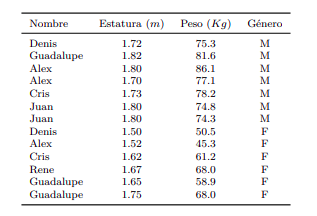
\includegraphics[width=.6\linewidth]{excercise1}
	  	\label{fig1}
	  \end{figure}
  \paragraph{} Entrena un clasificador bayesiano ingenuo usando estimación por máxima verosimilitud y otro usando estimación por máximo a posteriori. Reporta los parámetros que obtuviste en ambos casos y usa los clasificadores entrenados para predecir la clase de los siguientes vectores: x1 = (Rene, 1.68, 65), x2 = (Guadalupe, 1.75, 80), x3 = (Denis, 1.80, 79), x4 = (Alex, 190, 85) y x5 = (Cris, 165, 70).
  Describe de forma detallada el procedimiento que seguiste tanto en el entrenamiento como en la predicción y discute los resultados obtenidos.
  Para el entrenamiento del clasificador por máximo a posteriori considera los siguientes valores
  para las distribuciones correspondientes:
	  \begin{figure}[h!]
	  	\centering
	  	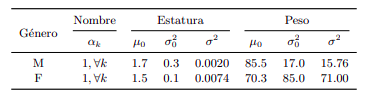
\includegraphics[width=.6\linewidth]{ex1_002}
	  	\label{fig2}
	  \end{figure}
  \clearpage
  \pagebreak
 \subsection{Estimador por máxima verosimilitud}
 \paragraph{} Los atributos son: \textbf{nombre}, \textbf{estatura} y \textbf{peso}, y la clase es \textbf{género}.\\
 \subsubsection{Atributo \textit{Nombre}}
 \paragraph{} Para el \textbf{nombre} podemos asumir una distribución categórica:
  \begin{equation}
  \begin{split}
  X_{nombre}^{(i)}\sim Cat(X_{nombre}^{(i)};q)\\
  \end{split}
  \end{equation}
  Donde las categorías son los nombres y los podemos enumerar:\\
  Denis - 1, Guadalupe - 2, Alex - 3, Cris - 4, Juan - 5, Rene - 6.\\
  \paragraph{}Y así con los nombres de 1 a 6 podemos definir a $Cat(X_{nombre}^{(i)};q)$ como:\\
  \begin{equation}
  \begin{split}
  Cat(X_{nombre}^{(i)};q) = \prod_{k=1}^{6}q_{k}^{[x_{nombre}^{(i)}=k ]}\\
  \end{split}
  \end{equation}
  Donde podemos estimar a $q_k$ usando el estimador de máxima verosimilitud como:
  \begin{equation}
  \begin{split}
  \hat{q}_k =& \frac{c_k}{n} \\ 
  \text{Donde $c_k$:}&\\
  c_k =& \sum_{i = 1}^{n}{[x^{(i)}_{nombre}=k]}
  \end{split}
  \end{equation}
  Así podemos estimar el parámetro para la primer categoría:\\
  \begin{equation}
  \begin{split}
  	\text{Para la clase \textbf{Femenino}}:\\
  	c_{1F} &= \sum_{i = 1}^{13}{[x^{(i)}_{nombre}=1 \text{ y $x^{(i)}$ es de la clase Femenino}]}\\
  	&= 0 + 0 + 0 + 0 + 0 + 0 + 0 + 0 + 1 + 0 + 0 + 0 + 0 + 0\\
  	&= 1\\
  \hat{q}_{(1|F)} =& \frac{1}{6} \\ 
  \text{Para la clase \textbf{Masculino}}:\\
  c_{1M} &= \sum_{i = 1}^{13}{[x^{(i)}_{nombre}=1 \text{ y $x^{(i)}$ es de la clase Masculino}]}\\
  &= 1 + 0 + 0 + 0 + 0 + 0 + 0 + 0 + 0 + 0 + 0 + 0 + 0 + 0\\
  &= 1\\
  \hat{q}_{(1|M)} =& \frac{1}{7} \\
  \end{split}
  \end{equation}
  Y de la misma forma para las categorías restantes:
  \begin{equation}
  \begin{split}
  c_{2F} = 2, \; \hat{q}_{(2|F)} = \frac{2}{6}, \; c_{2M} = 1, \; \hat{q}_{(2|M)} = \frac{1}{7} \; \; \; \; \; \; \; \; \; \; \; \; &  c_{3F} = 1, \; \hat{q}_{(3|F)} = \frac{1}{6}, \; c_{3M} = 2, \; \hat{q}_{(3|M)} = \frac{2}{7}\\
  c_{4F} = 1, \; \hat{q}_{(4|F)} = \frac{1}{6}, \; c_{4M} = 1, \; \hat{q}_{(4|M)} = \frac{1}{7} \; \; \; \; \; \; \; \; \; \; \; \; &  c_{5F} = 0, \; \hat{q}_{(5|F)} = \frac{0}{6} = 0, \; c_{5M} = 2, \; \hat{q}_{(5|M)} = \frac{2}{7}\\ 
  c_{6F} = 1, \; \hat{q}_{(6|F)} = \frac{1}{6}, \;c_{6M} = 0, \; \hat{q}_{(6|M)} = \frac{0}{7} = 0\\
  \end{split}
  \end{equation}
  \subsubsection{Atributo Estatura}
  \paragraph{}Para la \textbf{estatura} podemos asumir una distribución normal:
  \begin{equation}
  \begin{split}
  X_{estatura}^{(i)}\sim \mathcal{N}(X_{estatura}^{(i)};\mu;\sigma^2)\\
  \end{split}
  \end{equation}
  Donde $\mathcal{N}(X_{estatura}^{(i)};\mu;\sigma^2)$ se define como:\\
  \begin{equation}
  \begin{split}
  \mathcal{N}(X_{estatura}^{(i)};\mu;\sigma^2) =& \frac{1}{\sqrt{2\pi\sigma^2}}e^{\frac{-(x^{(i)} - \mu)^2}{2\sigma^2}}\\
  \end{split}
  \end{equation}
  Donde podemos estimar a $\mu$ y a $\sigma$ usando el estimador de máxima verosimilitud como:
  \paragraph{} Para la clase \textbf{Femenino}:
  \begin{equation}
  \begin{split}
  \hat{\mu}_{F}&=\frac{1}{n}\sum_{i=1}^{n}{x_{estatura}^{(i)}}\\
  &=\frac{1}{6}(1.50 + 1.52 + 1.62 + 1.67 + 1.65 + 1.75)\\
   &=\frac{1}{6}(9.71)\\
   &= 1.618\bar{3}\\
  \end{split}
  \end{equation}
  \begin{equation}
  \begin{split}
  \hat{\sigma}^2_F&=\frac{1}{n}\sum_{i=1}^{n}{(x_{estatura}^{(i)} - \hat{\mu})^2}\\
  &=\frac{1}{6}[(1.50-1.618\bar{3})^2 + (1.52-1.618\bar{3})^2  + \dots + (1.75-1.618\bar{3})^2)]\\
  &=\frac{1}{6}[0.014003 + 0.009669 + 0.000002\bar{7} + \dots + 0.0173361111]\\
  &=\frac{1}{6}[0.04468\bar{3}]\\
  &= 0.007447\bar{2}\\
  \end{split}
  \end{equation}
  \paragraph{} Para la clase \textbf{Masculino}:
  \begin{equation}
  \begin{split}
  \hat{\mu}_{M}&=\frac{1}{n}\sum_{i=1}^{n}{x_{estatura}^{(i)}}\\
  &=\frac{1}{7}(1.72 + 1.82 + 1.80 + 1.70 + 1.73 + 1.80 + 1.80)\\
  &=\frac{1}{7}(12.37)\\
  &= 1.7671428571428571\\
  \end{split}
  \end{equation}
  \begin{equation}
  \begin{split}
  \hat{\sigma}^2_M&=\frac{1}{n}\sum_{i=1}^{n}{(x_{estatura}^{(i)} - \hat{\mu})^2}\\
  &=\frac{1}{7}[(1.72-1.76714)^2 + (1.82-1.76714)^2  + \dots + (1.80-1.76714)^2)]\\
  &=\frac{1}{7}[0.00222245 + 0.00279388 + 0.00107959 + \dots + 0.00107959]\\
  &=\frac{1}{7}[0.014142857142857169]\\
  &= 0.0020204081632653097\\
  \end{split}
  \end{equation}
  \subsubsection{Atributo Peso}
  \paragraph{}Para el \textbf{peso} podemos asumir una distribución normal:
  \begin{equation}
  \begin{split}
  X_{peso}^{(i)}\sim \mathcal{N}(X_{peso}^{(i)};\mu;\sigma^2)\\
  \end{split}
  \end{equation}
  Donde $\mathcal{N}(X_{peso}^{(i)};\mu;\sigma^2)$ se define como:\\
  \begin{equation}
  \begin{split}
  \mathcal{N}(X_{peso}^{(i)};\mu;\sigma^2) =& \frac{1}{\sqrt{2\pi\sigma^2}}e^{\frac{-(x^{(i)} - \mu)^2}{2\sigma^2}}\\
  \end{split}
  \end{equation}
  Donde podemos estimar a $\mu$ y a $\sigma$ usando el estimador de máxima verosimilitud como:
  \paragraph{} Para la clase \textbf{Femenino}:
  \begin{equation}
  \begin{split}
  \hat{\mu}_{F}&=\frac{1}{n}\sum_{i=1}^{n}{x_{peso}^{(i)}}\\
  &=\frac{1}{6}(50.5 + 45.3 + 61.2 + 68.0 + 58.9 + 68.0)\\
  &=\frac{1}{6}(351.9)\\
  &= 58.65\\
  \end{split}
  \end{equation}
  \begin{equation}
  \begin{split}
  \hat{\sigma}_F^2&=\frac{1}{n}\sum_{i=1}^{n}{(x_{peso}^{(i)} - \hat{\mu})^2}\\
  &=\frac{1}{6}[(50.5-58.65)^2 + (45.3-58.65)^2  + \dots + (68.0-58.65)^2)]\\
  &=\frac{1}{6}[66.42250 + 178.2225 + 6.502500 + \dots + 87.42250]\\
  &=\frac{1}{6}[426.055]\\
  &= 71.00916\bar{7}\\
  \end{split}
  \end{equation}
  \paragraph{} Para la clase \textbf{Masculino}:
  \begin{equation}
  \begin{split}
  \hat{\mu}_{M}&=\frac{1}{n}\sum_{i=1}^{n}{x_{peso}^{(i)}}\\
  &=\frac{1}{7}(75.3 + 81.6 + 86.1 + 77.1 + 78.2 + 74.8 + 74.3)\\
  &=\frac{1}{7}(547.4)\\
  &= 78.2\\
  \end{split}
  \end{equation}
  \begin{equation}
  \begin{split}
  \hat{\sigma}_M^2&=\frac{1}{n}\sum_{i=1}^{n}{(x_{peso}^{(i)} - \hat{\mu})^2}\\
  &=\frac{1}{7}[(75.3-78.2)^2 + (81.6-78.2)^2  + \dots + (74.3-78.2)^2)]\\
  &=\frac{1}{7}[8.41 + 11.56 + 62.41 + \dots + 15.21]\\
  &=\frac{1}{7}[110.36]\\
  &= 15.7657142857142\\
  \end{split}
  \end{equation}
  \clearpage
  \pagebreak
  \subsubsection{Género}
  Para la clase (Género) podemos asumir una distribución Bernoulli:
  \begin{equation}
  \begin{split}
  Y^{(i)}\sim Ber(Y^{(i)};q)\\
  \end{split}
  \end{equation}
  Donde $Ber(Y^{(i)};q)$ se define como:\\
  \begin{equation}
  	\begin{split}
  		Ber(Y^{(i)};q)&= q^C(1 - q)^{1-C}\\
  		C &= [y = \text{clase}]
  	\end{split}
  \end{equation}
 Donde podemos estimar a $q$ usando el estimador de máxima verosimilitud como:\\
 \paragraph{}Para la clase \textbf{Femenino}:
 \begin{equation}
 	\begin{split}
 		\hat{q}_F &= \frac{N_F}{N}\\
 		&= \frac{6}{13}\\
 	\end{split}
 \end{equation}
 \paragraph{}Para la clase \textbf{Masculino}:
 \begin{equation}
 \begin{split}
 \hat{q}_M &= \frac{N_M}{N}\\
 &= \frac{7}{13}\\
 \end{split}
 \end{equation}
 \clearpage
 \pagebreak
 \subsubsection{Uso del Estimador por Máxima Verosimilitud}
 \paragraph{} Clasificaremos al vector de entrada con base en la siguiente ecuación:
 \begin{equation}
 	\begin{split}
 		C &= \text{max arg}_{C\in\{F,M\}} \{ P(X|C)P(C)\} \\
 		&\text{Donde las probabilidades de cada parametro al ser independientes se multiplicaran}\\
 		&= \text{max arg}_{C\in\{F,M\}} \{ P(C) P(X_{nombre}|C)P(X_{estatura}|C)P(X_{peso}|C)\}
 	\end{split}
 \end{equation}
 \paragraph{Prueba 1: }x1= (Rene, 1.68, 65)
 \paragraph{}Probabilidad de que sea \textbf{Femenino}:\\
 \begin{equation}
 \begin{split}
 P(F|x1) &\propto P(F) \times P(x1_{nombre}|F) \times P(x1_{estatura}|F) \times P(x1_{peso}|F) \\
 &\propto (\frac{6}{13}) \times (\frac{1}{6}) \times (\frac{1}{\sqrt{2\pi\hat{\sigma}_{\text{estatura}|F}^2}}e^{\frac{-(x1 - \hat{\mu}_{\text{estatura}|F})^2}{2\hat{\sigma}_{\text{estatura}|F}^2}}) \times (\frac{1}{\sqrt{2\pi\hat{\sigma}_{\text{peso}|F}^2}}e^{\frac{-(x1 - \hat{\mu}_{\text{peso}|F})^2}{2\hat{\sigma}_{\text{peso}|F}^2}}) \\
 &\propto (\frac{6}{13}) \times (\frac{1}{6}) \times (3.4113057085685545) \times (0.03411194570280468) \\
 &\propto 0.00895125193125832 \\
 &\propto 0.89512\% \\
 \end{split}
 \end{equation}
 \paragraph{}Probabilidad de que sea \textbf{Masculino}:\\
 \begin{equation}
 \begin{split}
 P(M|x1) &\propto P(M) \times P(x1_{nombre}|M) \times P(x1_{estatura}|M) \times P(x1_{peso}|M) \\
 &\propto (\frac{7}{13}) \times (0) \times (\frac{1}{\sqrt{2\pi\hat{\sigma}_{\text{estatura}|M}^2}}e^{\frac{-(x1 - \hat{\mu}_{\text{estatura}|M})^2}{2\hat{\sigma}_{\text{estatura}|F}^2}}) \times (\frac{1}{\sqrt{2\pi\hat{\sigma}_{\text{peso}|M}^2}}e^{\frac{-(x1 - \hat{\mu}_{\text{peso}|M})^2}{2\hat{\sigma}_{\text{peso}|M}^2}}) \\
 &\propto (\frac{7}{13}) \times (0) \times (1.641140586274889) \times (0.03411194570280468) \\
 &\propto 0 \\
 &\propto 0 \% \\
 \end{split}
 \end{equation}
 Así para el caso 1 la clasificación sería \textbf{Femenino} puesto que $0.89512\% > 0\%$.\\
 \clearpage
 \pagebreak
 \paragraph{Prueba 2: }x2= (Guadalupe, 1.75, 80)
 \paragraph{}Probabilidad de que sea \textbf{Femenino}:\\
 \begin{equation}
 \begin{split}
 P(F|x2) &\propto P(F) \times P(x2_{nombre}|F) \times P(x2_{estatura}|F) \times P(x2_{peso}|F) \\
 &\propto (\frac{6}{13}) \times (\frac{2}{6}) \times (\frac{1}{\sqrt{2\pi\hat{\sigma}_{\text{estatura}|F}^2}}e^{\frac{-(x2 - \hat{\mu}_{\text{estatura}|F})^2}{2\hat{\sigma}_{\text{estatura}|F}^2}}) \times (\frac{1}{\sqrt{2\pi\hat{\sigma}_{\text{peso}|F}^2}}e^{\frac{-(x2 - \hat{\mu}_{\text{peso}|F})^2}{2\hat{\sigma}_{\text{peso}|F}^2}}) \\
 &\propto (\frac{6}{13}) \times (\frac{2}{6}) \times (1.599858146833577) \times (0.0029789834817996216) \\
 &\propto 0.0007332232296368892 \\
 &\propto 0.073322\% \\
 \end{split}
 \end{equation}
 \paragraph{}Probabilidad de que sea \textbf{Masculino}:\\
 \begin{equation}
 \begin{split}
 P(M|x2) &\propto P(M) \times P(x2_{nombre}|M) \times P(x2_{estatura}|M) \times P(x2_{peso}|M) \\
 &\propto (\frac{7}{13}) \times (\frac{1}{7}) \times (\frac{1}{\sqrt{2\pi\hat{\sigma}_{\text{estatura}|M}^2}}e^{\frac{-(x2 - \hat{\mu}_{\text{estatura}|M})^2}{2\hat{\sigma}_{\text{estatura}|F}^2}}) \times (\frac{1}{\sqrt{2\pi\hat{\sigma}_{\text{peso}|M}^2}}e^{\frac{-(x2 - \hat{\mu}_{\text{peso}|M})^2}{2\hat{\sigma}_{\text{peso}|M}^2}}) \\
 &\propto (\frac{7}{13}) \times (\frac{1}{7}) \times (7.720478376796198) \times (0.0029789834817996216) \\
 &\propto 0.050585966030299065 \\
 &\propto 5.05859 \% \\
 \end{split}
 \end{equation}
 Así para el caso 2 la clasificación sería \textbf{Masculino} puesto que $5.05859\% > 0.073322\%$.\\
 \paragraph{Prueba 3: }x3= (Denis, 1.80, 79)
 \paragraph{}Probabilidad de que sea \textbf{Femenino}:\\
 \begin{equation}
 \begin{split}
 P(F|x3) &\propto P(F) \times P(x3_{nombre}|F) \times P(x3_{estatura}|F) \times P(x3_{peso}|F) \\
 &\propto (\frac{6}{13}) \times (\frac{1}{6}) \times (\frac{1}{\sqrt{2\pi\hat{\sigma}_{\text{estatura}|F}^2}}e^{\frac{-(x3 - \hat{\mu}_{\text{estatura}|F})^2}{2\hat{\sigma}_{\text{estatura}|F}^2}}) \times (\frac{1}{\sqrt{2\pi\hat{\sigma}_{\text{peso}|F}^2}}e^{\frac{-(x3 - \hat{\mu}_{\text{peso}|F})^2}{2\hat{\sigma}_{\text{peso}|F}^2}}) \\
 &\propto (\frac{6}{13}) \times (\frac{1}{6}) \times (0.6658947606886298) \times (0.003804820622723802) \\
 &\propto 0.00019489308600244848 \\
 &\propto 0.019489\% \\
 \end{split}
 \end{equation}
 \paragraph{}Probabilidad de que sea \textbf{Masculino}:\\
 \begin{equation}
 \begin{split}
 P(M|x3) &\propto P(M) \times P(x3_{nombre}|M) \times P(x3_{estatura}|M) \times P(x3_{peso}|M) \\
 &\propto (\frac{7}{13}) \times (\frac{1}{7}) \times (\frac{1}{\sqrt{2\pi\hat{\sigma}_{\text{estatura}|M}^2}}e^{\frac{-(x3 - \hat{\mu}_{\text{estatura}|M})^2}{2\hat{\sigma}_{\text{estatura}|F}^2}}) \times (\frac{1}{\sqrt{2\pi\hat{\sigma}_{\text{peso}|M}^2}}e^{\frac{-(x3 - \hat{\mu}_{\text{peso}|M})^2}{2\hat{\sigma}_{\text{peso}|M}^2}}) \\
 &\propto (\frac{7}{13}) \times (\frac{1}{7}) \times (6.53524385337116) \times (0.003804820622723802) \\
 &\propto 0.04595604066151125 \\
 &\propto 4.5956 \% \\
 \end{split}
 \end{equation}
 Así para el caso 3 la clasificación sería \textbf{Masculino} puesto que $4.5956\% > 0.019489\%$.\\
 \paragraph{Prueba 4: }x4= (Alex, 1.90, 85)
 \paragraph{}Probabilidad de que sea \textbf{Femenino}:\\
 \begin{equation}
 \begin{split}
 P(F|x4) &\propto P(F) \times P(x4_{nombre}|F) \times P(x4_{estatura}|F) \times P(x4_{peso}|F) \\
 &\propto (\frac{6}{13}) \times (\frac{1}{6}) \times (\frac{1}{\sqrt{2\pi\hat{\sigma}_{\text{estatura}|F}^2}}e^{\frac{-(x4 - \hat{\mu}_{\text{estatura}|F})^2}{2\hat{\sigma}_{\text{estatura}|F}^2}}) \times (\frac{1}{\sqrt{2\pi\hat{\sigma}_{\text{peso}|F}^2}}e^{\frac{-(x4 - \hat{\mu}_{\text{peso}|F})^2}{2\hat{\sigma}_{\text{peso}|F}^2}}) \\
 &\propto (\frac{6}{13}) \times (\frac{1}{6}) \times (0.04983987374064044) \times (0.0007349997821943831) \\
 &\propto 0.0000028178689495358674 \\
 &\propto 0.00028178\% \\
 \end{split}
 \end{equation}
 \paragraph{}Probabilidad de que sea \textbf{Masculino}:\\
 \begin{equation}
 \begin{split}
 P(M|x4) &\propto P(M) \times P(x4_{nombre}|M) \times P(x4_{estatura}|M) \times P(x4_{peso}|M) \\
 &\propto (\frac{7}{13}) \times (\frac{2}{7}) \times (\frac{1}{\sqrt{2\pi\hat{\sigma}_{\text{estatura}|M}^2}}e^{\frac{-(x4 - \hat{\mu}_{\text{estatura}|M})^2}{2\hat{\sigma}_{\text{estatura}|F}^2}}) \times (\frac{1}{\sqrt{2\pi\hat{\sigma}_{\text{peso}|M}^2}}e^{\frac{-(x4 - \hat{\mu}_{\text{peso}|M})^2}{2\hat{\sigma}_{\text{peso}|M}^2}}) \\
 &\propto (\frac{7}{13}) \times (\frac{2}{7}) \times (0.1943796927071898) \times (0.0007349997821943831) \\
 &\propto 0.0007914420714764275 \\
 &\propto 0.079144 \% \\
 \end{split}
 \end{equation}
 Así para el caso 3 la clasificación sería \textbf{Masculino} puesto que $0.079144\% > 0.00028178\%$.\\
 \paragraph{Prueba 5: }x5= (Cris, 1.65, 70)
 \paragraph{}Probabilidad de que sea \textbf{Femenino}:\\
 \begin{equation}
 \begin{split}
 P(F|x5) &\propto P(F) \times P(x5_{nombre}|F) \times P(x5_{estatura}|F) \times P(x5_{peso}|F) \\
 &\propto (\frac{6}{13}) \times (\frac{1}{6}) \times (\frac{1}{\sqrt{2\pi\hat{\sigma}_{\text{estatura}|F}^2}}e^{\frac{-(x5 - \hat{\mu}_{\text{estatura}|F})^2}{2\hat{\sigma}_{\text{estatura}|F}^2}}) \times (\frac{1}{\sqrt{2\pi\hat{\sigma}_{\text{peso}|F}^2}}e^{\frac{-(x5 - \hat{\mu}_{\text{peso}|F})^2}{2\hat{\sigma}_{\text{peso}|F}^2}}) \\
 &\propto (\frac{6}{13}) \times (\frac{1}{6}) \times (3.989847809495735) \times (0.020294471017724632) \\
 &\propto 0.006228603902687947 \\
 &\propto 0.62286\% \\
 \end{split}
 \end{equation}
 \paragraph{}Probabilidad de que sea \textbf{Masculino}:\\
 \begin{equation}
 \begin{split}
 P(M|x5) &\propto P(M) \times P(x5_{nombre}|M) \times P(x5_{estatura}|M) \times P(x5_{peso}|M) \\
 &\propto (\frac{7}{13}) \times (\frac{1}{7}) \times (\frac{1}{\sqrt{2\pi\hat{\sigma}_{\text{estatura}|M}^2}}e^{\frac{-(x5 - \hat{\mu}_{\text{estatura}|M})^2}{2\hat{\sigma}_{\text{estatura}|F}^2}}) \times (\frac{1}{\sqrt{2\pi\hat{\sigma}_{\text{peso}|M}^2}}e^{\frac{-(x5 - \hat{\mu}_{\text{peso}|M})^2}{2\hat{\sigma}_{\text{peso}|M}^2}}) \\
 &\propto (\frac{7}{13}) \times (\frac{1}{7}) \times (0.4472629865983849) \times (0.020294471017724632) \\
 &\propto 0.0005144939695681998 \\
 &\propto 0.051449 \% \\
 \end{split}
 \end{equation}
 Así para el caso 3 la clasificación sería \textbf{Femenino} puesto que $0.62286\% > 0.051449\%$.\\
 \subsection{Estimador por máximo a posteriori}
 \paragraph{}Los atributos son: \textbf{nombre}, \textbf{estatura} y \textbf{peso}, y la clase es \textbf{género}.\\
 \subsubsection{Atributo \textit{Nombre}}
 \paragraph{} Para el \textbf{nombre} podemos asumir una distribución categórica:
 \begin{equation}
 \begin{split}
 X_{nombre}^{(i)}\sim Cat(X_{nombre}^{(i)};q)\\
 \end{split}
 \end{equation}
 Donde las categorías son los nombres y los podemos enumerar:\\
 Denis - 1, Guadalupe - 2, Alex - 3, Cris - 4, Juan - 5, Rene - 6.\\
 \paragraph{}Y así con los nombres de 1 a 6 podemos definir a $Cat(X_{nombre}^{(i)};q)$ como:\\
 \begin{equation}
 \begin{split}
 Cat(X_{nombre}^{(i)};q) = \prod_{k=1}^{6}q_{k}^{[x_{nombre}^{(i)}=k ]}\\
 \end{split}
 \end{equation}
 Donde podemos estimar a $q_k$ usando el estimador MAP como:
 \begin{equation}
 \begin{split}
 \hat{q}_k =& \frac{c_k + \alpha_k - 1}{n - K + \sum_{i=1}^{K}{\alpha_i}} \\ 
 \text{Donde:}&\\
 \alpha_k =& 1,\; \forall k\\
 K =& \; 6\\
 n =& \; \text{numero elementos de la clase}\\
 c_k =& \sum_{i = 1}^{n}{[x^{(i)}_{nombre}=k]}
 \end{split}
 \end{equation}
 Así podemos estimar el parámetro para la primer categoría:\\
 \begin{equation}
 \begin{split}
 \text{Para la clase \textbf{Femenino}}:\\
 c_{1F} &= \sum_{i = 1}^{13}{[x^{(i)}_{nombre}=1 \text{ y $x^{(i)}$ es de la clase Femenino}]}\\
 &= 0 + 0 + 0 + 0 + 0 + 0 + 0 + 0 + 1 + 0 + 0 + 0 + 0 + 0\\
 &= 1\\
 \hat{q}_{(1|F)} &= \frac{1 + 1 - 1}{6 - 6 + \sum_{i=1}^{6}{1}} \\
 &= \frac{1 + 1 - 1}{6 - 6 + 6} \\  
 &= \frac{1}{6} \\
 \text{Para la clase \textbf{Masculino}}:\\
 c_{1M} &= \sum_{i = 1}^{13}{[x^{(i)}_{nombre}=1 \text{ y $x^{(i)}$ es de la clase Masculino}]}\\
 &= 1 + 0 + 0 + 0 + 0 + 0 + 0 + 0 + 0 + 0 + 0 + 0 + 0 + 0\\
 &= 1\\
 \hat{q}_{(1|M)} &= \frac{1 + 1 - 1}{7 - 6 + \sum_{i=1}^{6}{1}} \\
 &= \frac{1 + 1 - 1}{7 - 6 + 6} \\  
 &= \frac{1}{7} \\
 \end{split}
 \end{equation}
 Y de la misma forma para las categorías restantes:
 \begin{equation}
 \begin{split}
 c_{2F} = 2, \; \hat{q}_{(2|F)} = \frac{2}{6}, \; c_{2M} = 1, \; \hat{q}_{(2|M)} = \frac{1}{7} \; \; \; \; \; \; \; \; \; \; \; \; &  c_{3F} = 1, \; \hat{q}_{(3|F)} = \frac{1}{6}, \; c_{3M} = 2, \; \hat{q}_{(3|M)} = \frac{2}{7}\\
 c_{4F} = 1, \; \hat{q}_{(4|F)} = \frac{1}{6}, \; c_{4M} = 1, \; \hat{q}_{(4|M)} = \frac{1}{7} \; \; \; \; \; \; \; \; \; \; \; \; &  c_{5F} = 0, \; \hat{q}_{(5|F)} = \frac{0}{6} = 0, \; c_{5M} = 2, \; \hat{q}_{(5|M)} = \frac{2}{7}\\ 
 c_{6F} = 1, \; \hat{q}_{(6|F)} = \frac{1}{6}, \;c_{6M} = 0, \; \hat{q}_{(6|M)} = \frac{0}{7} = 0\\
 \end{split}
 \end{equation}
 \subsubsection{Atributo Estatura}
 \paragraph{}Para la \textbf{estatura} podemos asumir una distribución normal:
 \begin{equation}
 \begin{split}
 X_{estatura}^{(i)}\sim \mathcal{N}(X_{estatura}^{(i)};\mu;\sigma^2)\\
 \end{split}
 \end{equation}
 Donde $\mathcal{N}(X_{estatura}^{(i)};\mu;\sigma^2)$ se define como:\\
 \begin{equation}
 \begin{split}
 \mathcal{N}(X_{estatura}^{(i)};\mu;\sigma^2) =& \frac{1}{\sqrt{2\pi\sigma^2}}e^{\frac{-(x^{(i)} - \mu)^2}{2\sigma^2}}\\
 \end{split}
 \end{equation}
 Donde $\sigma_F^2 = 0.0074$ y $\sigma_M^2 = 0.0020$, podemos estimar a $\mu$ para cada clase usando el estimador MAP como:
 \paragraph{} Para la clase \textbf{Femenino}:
 \begin{equation}
 \begin{split}
 \hat{\mu}_{F}&=\frac{\sigma_{0F}^2(\sum_{i=1}^{n}{x_{estatura}^{(i)}}) + \sigma_F^2\mu_{0F} }{\sigma_{0F}^2n + \sigma_F^2}\\
 &=\frac{0.1\times(\sum_{i=1}^{n}{x_{estatura}^{(i)}}) + (0.0074\times 1.5) }{(0.1 \times 6) + 0.0074}\\
 &=\frac{0.1\times(1.50 + 1.52 + 1.62 + 1.67 + 1.65 + 1.75) + (0.0111) }{0.6074}\\
 &=\frac{(0.1\times 9.71) + (0.0111) }{0.6074}\\
 &=\frac{0.971 + 0.0111 }{0.6074}\\
 &=\frac{0.9821}{0.6074}\\
 &= 1.6168916694106026\\
 \end{split}
 \end{equation}
\paragraph{} Para la clase \textbf{Masculino}:
\begin{equation}
\begin{split}
\hat{\mu}_{M}&=\frac{\sigma_{0M}^2(\sum_{i=1}^{n}{x_{estatura}^{(i)}}) + \sigma_M^2\mu_{0M} }{\sigma_{0M}^2n + \sigma_M^2}\\
&=\frac{0.3\times(\sum_{i=1}^{n}{x_{estatura}^{(i)}}) + (0.0020\times 1.7) }{(0.3 \times 7) + 0.0020}\\
&=\frac{0.3\times(1.72 + 1.82 + 1.80 + 1.70 + 1.73 + 1.80 + 1.80) + (0.0034) }{2.102}\\
&=\frac{(0.3\times 12.37) + (0.0034) }{2.102}\\
&=\frac{3.711 + 0.0034 }{2.102}\\
&=\frac{3.7144}{2.102}\\
&= 1.7670789724072313\\
\end{split}
\end{equation}
 \subsubsection{Atributo Peso}
\paragraph{}Para el \textbf{peso} podemos asumir una distribución normal:
\begin{equation}
\begin{split}
X_{peso}^{(i)}\sim \mathcal{N}(X_{peso}^{(i)};\mu;\sigma^2)\\
\end{split}
\end{equation}
Donde $\mathcal{N}(X_{peso}^{(i)};\mu;\sigma^2)$ se define como:\\
\begin{equation}
\begin{split}
\mathcal{N}(X_{peso}^{(i)};\mu;\sigma^2) =& \frac{1}{\sqrt{2\pi\sigma^2}}e^{\frac{-(x^{(i)} - \mu)^2}{2\sigma^2}}\\
\end{split}
\end{equation}
Donde $\sigma_F^2 = 71.00$ y $\sigma_M^2 = 15.76$, podemos estimar a $\mu$ para cada clase usando el estimador MAP como:
\paragraph{} Para la clase \textbf{Femenino}:
\begin{equation}
\begin{split}
\hat{\mu}_{F}&=\frac{\sigma_{0F}^2(\sum_{i=1}^{n}{x_{peso}^{(i)}}) + \sigma_F^2\mu_{0F} }{\sigma_{0F}^2n + \sigma_F^2}\\
&=\frac{85\times(\sum_{i=1}^{n}{x_{peso}^{(i)}}) + (71.0\times 70.3) }{(85 \times 6) + 71.0}\\
&=\frac{85.5\times(50.5 + 45.3 + 61.2 + 68.0 + 58.9 + 68.0) + (4991.3) }{581}\\
&=\frac{(85\times 351.9) + (4991.3) }{581}\\
&=\frac{29911.5 + 4991.3 }{581}\\
&=\frac{34902.8}{581}\\
&= 60.073666092943206\\
\end{split}
\end{equation}
\paragraph{} Para la clase \textbf{Masculino}:
\begin{equation}
\begin{split}
\hat{\mu}_{M}&=\frac{\sigma_{0M}^2(\sum_{i=1}^{n}{x_{peso}^{(i)}}) + \sigma_M^2\mu_{0M} }{\sigma_{0M}^2n + \sigma_M^2}\\
&=\frac{17.0\times(\sum_{i=1}^{n}{x_{peso}^{(i)}}) + (15.76\times 85.5) }{(17.0 \times 7) + 15.76}\\
&=\frac{17.0\times(75.3 + 81.6 + 86.1 + 77.1 + 78.2 + 74.8 + 74.3) + (1347.48) }{134.76}\\
&=\frac{(17.0\times 547.4) + (1347.48) }{134.76}\\
&=\frac{9305.8 + 1347.48}{134.76}\\
&=\frac{10653.28}{134.76}\\
&= 79.0537251409914\\
\end{split}
\end{equation}
\subsubsection{Género}
Para la clase (Género) podemos asumir una distribución Bernoulli:
\begin{equation}
\begin{split}
Y^{(i)}\sim Ber(Y^{(i)};q)\\
\end{split}
\end{equation}
Donde $Ber(Y^{(i)};q)$ se define como:\\
\begin{equation}
\begin{split}
Ber(Y^{(i)};q)&= q^C(1 - q)^{1-C}\\
C &= [y = \text{clase}]
\end{split}
\end{equation}
Donde podemos estimar a $q$ usando el estimador MAP con los hyperparametros equivalentes al suavizado de laplace $\alpha_F = 2$, $\alpha_M = 2$, $\beta_F = 6$y $\beta_M = 7$ como:\\
\paragraph{}Para la clase \textbf{Femenino}:
\begin{equation}
\begin{split}
\hat{q}_F &= \frac{N_F + \alpha_F - 1}{N + \beta_F + \alpha_F - 2}\\
&= \frac{6 + 2 - 1}{13 + 2 + 2 - 2}\\
&= \frac{7}{15}\\
\end{split}
\end{equation}
\paragraph{}Para la clase \textbf{Masculino}:
\begin{equation}
\begin{split}
\hat{q}_M &= \frac{N_M + \alpha_M - 1}{N + \beta_M + \alpha_M - 2}\\
&= \frac{7 + 2 - 1}{13 + 2 + 2 - 2}\\
&= \frac{8}{15}\\
\end{split}
\end{equation}
\clearpage
\pagebreak
\subsubsection{Uso del Clasificador MAP}
\paragraph{} Clasificaremos al vector de entrada con base en la siguiente ecuación:
\begin{equation}
\begin{split}
C &= \text{max arg}_{C\in\{F,M\}} \{ P(X|C)P(C)\} \\
&\text{Donde las probabilidades de cada parametro al ser independientes se multiplicaran}\\
&= \text{max arg}_{C\in\{F,M\}} \{ P(C) P(X_{nombre}|C)P(X_{estatura}|C)P(X_{peso}|C)\}
\end{split}
\end{equation}
\paragraph{Prueba 1: }x1= (Rene, 1.68, 65)
\paragraph{}Probabilidad de que sea \textbf{Femenino}:\\
\begin{equation}
\begin{split}
P(F|x1) &\propto P(F) \times P(x1_{nombre}|F) \times P(x1_{estatura}|F) \times P(x1_{peso}|F) \\
&\propto (\frac{7}{19}) \times (\frac{1}{6}) \times (\frac{1}{\sqrt{2\pi\hat{\sigma}_{\text{estatura}|F}^2}}e^{\frac{-(x1 - \hat{\mu}_{\text{estatura}|F})^2}{2\hat{\sigma}_{\text{estatura}|F}^2}}) \times (\frac{1}{\sqrt{2\pi\hat{\sigma}_{\text{peso}|F}^2}}e^{\frac{-(x1 - \hat{\mu}_{\text{peso}|F})^2}{2\hat{\sigma}_{\text{peso}|F}^2}}) \\
&\propto (\frac{7}{19}) \times (\frac{1}{6}) \times (3.543448351597527) \times (0.03990772866850168) \\
&\propto 0.008683130066358118 \\
&\propto 0.86831\% \\
\end{split}
\end{equation}
\paragraph{}Probabilidad de que sea \textbf{Masculino}:\\
\begin{equation}
\begin{split}
P(M|x1) &\propto P(M) \times P(x1_{nombre}|M) \times P(x1_{estatura}|M) \times P(x1_{peso}|M) \\
&\propto (\frac{2}{5}) \times (0) \times (\frac{1}{\sqrt{2\pi\hat{\sigma}_{\text{estatura}|M}^2}}e^{\frac{-(x1 - \hat{\mu}_{\text{estatura}|M})^2}{2\hat{\sigma}_{\text{estatura}|F}^2}}) \times (\frac{1}{\sqrt{2\pi\hat{\sigma}_{\text{peso}|M}^2}}e^{\frac{-(x1 - \hat{\mu}_{\text{peso}|M})^2}{2\hat{\sigma}_{\text{peso}|M}^2}}) \\
&\propto (\frac{2}{5}) \times (0) \times (1.641140586274889) \times (0.03411194570280468) \\
&\propto 0 \\
&\propto 0 \% \\
\end{split}
\end{equation}
Así para el caso 1 la clasificación sería \textbf{Femenino} puesto que $0.89512\% > 0\%$.\\
\clearpage
\pagebreak
\section{SPAM}
\paragraph{}El ejercicio se encuentra en Colab:\\
\url{https://colab.research.google.com/drive/1UoK-5HRnuQeLQaa4__uYeaCvyKkcMMMD}
\section{Cáncer de seno}
\paragraph{}El ejercicio se encuentra en Colab:\\
\url{https://colab.research.google.com/drive/1UoK-5HRnuQeLQaa4__uYeaCvyKkcMMMD}  
\end{document}  